\documentclass[a4paper]{exam}
\usepackage{amsfonts,amsmath,amsthm}
\usepackage[a4paper]{geometry}
\usepackage{xcolor}
\usepackage{wasysym}


\usepackage{amsfonts,amsmath,amsthm}
\usepackage{xcolor}
\usepackage{wasysym}

\usepackage{tikz}
\usepackage{tikz-qtree}


\newcommand\N{\ensuremath{\mathbb{N}}}
\newcommand\union{\cup}
\newcommand\interx{\cap}

\header{CS/MATH 113}{WC09: More on Induction}{Spring 2025}
\footer{}{Page \thepage\ of \numpages}{}
\runningheadrule
\runningfootrule

% \printanswers

\qformat{{\large\bf \thequestion. \thequestiontitle}\hfill}
\boxedpoints

\title{Weekly Challenge 10: Graphs}
\author{CS/MATH 113 Discrete Mathematics}
\date{Spring 2025}

\begin{document}
\maketitle



\begin{questions}
    \titledquestion{Permuting numbers} 
    In the year 3025 fascism is at the rise in the galactic empire. Political alliances are being formed. You as rebels want to break these alliances to kill off these ideologies before they take over every corner of the galaxy. 
    A faction is a group of people who have political alliances with each other. For example if Kirk is in alliance with Reinhard and Reinhard is in alliance with Paul then Kirk, Reinhard and Paul are in the same faction (even though Kirk and Paul are not in alliance themselves). Given any faction you want to break it into smaller factions.
    Your rebel forces captain Khubaib is a pacifist he thinks the best way to break these factions is to talk to people so that they break the alliance with some one. Khubaib is a master at persuasion he can talk to anyone convince them to break one of their alliances (in order for them to break more alliances Khubaib will have to talk to them again). Figure~\ref{1} shows an example of this. 
    Let $P$ be the smallest number of times Khubaib has to talk to someone to break a faction. 
    Munawar, who is the second in command in the rebels on the other hand knows how these factions work, by the time you guys are able to break a faction they would have already increased in size. He suggests to eliminate the people from factions (with any means necessary) so the faction breaks into smaller factions. Figure~\ref{2} shows an example of this. 
    Let $Q$ be the smallest number of people you have to eliminate in order to break the faction. 


    \begin{parts}
        \part You act as an arbitrator between Khubaib and Munawar. Prove or disprove that $P \geq Q$.
        \part You now want to take an idea about how many people are in each faction. A chain in a faction is a series of people $s_1, s_2, \dots s_n$ such that each person $s_i$ is in alliance with person $s_{i+1}$ and $s_1$ is in alliance with $s_n$ for each $i \in [n-1]$. 
        With your spies you have been able to find out that the smallest chain in any faction is of 4 people. And that everyone in each faction is in alliance with at least $m$ people. Sadly your spies were caught and they weren't able to deliver back any more information. But you studied Discrete Mathematics from Habib University a 1000 years ago so for you this information is sufficient. Prove or disprove that there are at least $2m$ people in each faction.
    \end{parts}
    %  factions fight for the control of the galaxy. People have 
    %  nation of TODO political alliances 
    \begin{solution}
        % Enter solution here.
    \end{solution}

    \begin{figure}[!tbh]
        \centering
        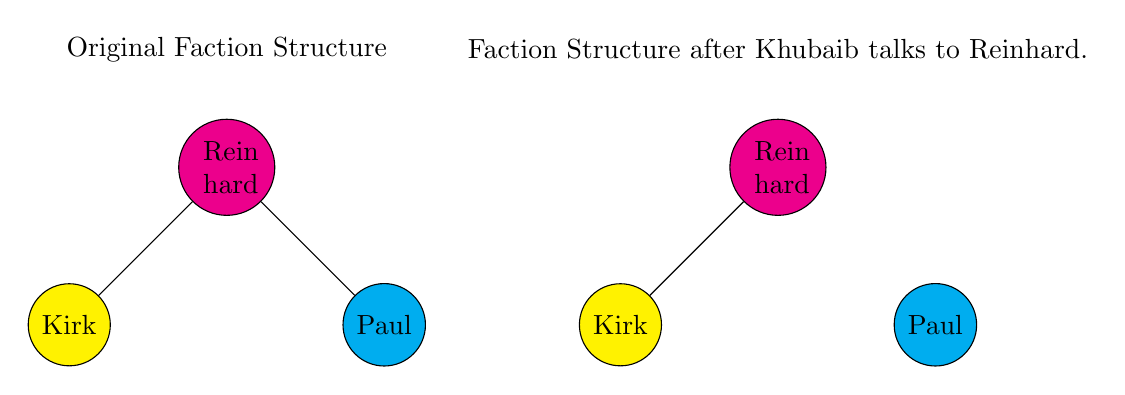
\begin{tikzpicture} 
            \node [] (L) at (2,3.5) {Original Faction Structure};
            \node [style={circle,draw, fill=yellow}] (A) at (0,0) {Kirk};
            \node [style={circle,draw,text width=6mm, fill = magenta}] (B) at (2,2) {Rein\\hard};
            \node [style={circle,draw, fill = cyan}] (C) at (4,0) {Paul};
            \draw (A) -- (B);
            \draw (B) -- (C);

            
            \node [] (L) at (9,3.5) {Faction Structure after Khubaib talks to Reinhard.};
            \node [style={circle,draw, fill = yellow}] (A1) at (7,0) {Kirk};
            \node [style={circle,draw,text width=6mm, fill = magenta}] (B1) at (9,2) {Rein\\hard};
            \node [style={circle,draw}, fill = cyan] (C1) at (11,0) {Paul};
            \draw (A1) -- (B1);


        \end{tikzpicture}
        \caption{Kirk is in alliance with Reinhard and Reinhard is in alliance with Paul. So Kirk, Reinhard and Paul form a faction. On the left we have the original faction structure then on right we have the faction structure after Khubaib talks to Reinhard and convince him to break his alliance with Paul.}
        \label{1}
    \end{figure}
        
%  \vspace{0.5cm}
\begin{figure}[!tbh]
    \centering
    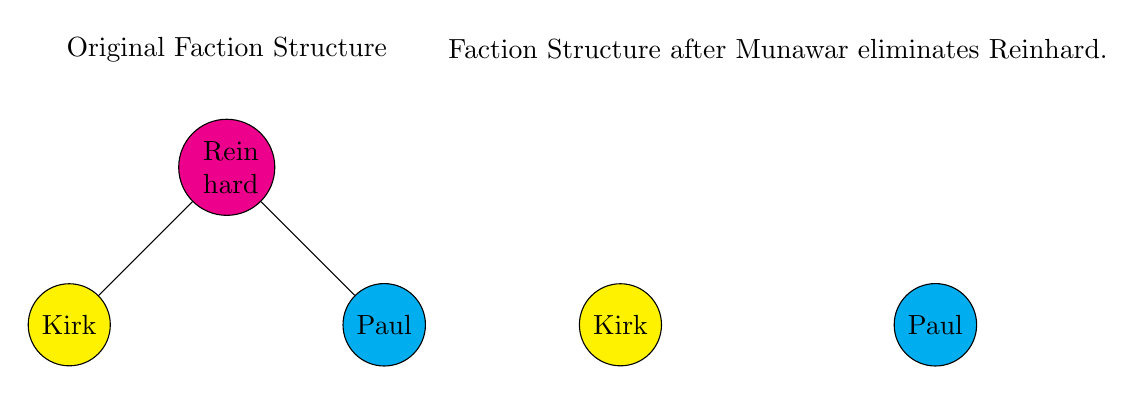
\begin{tikzpicture} 
        \node [] (L) at (2,3.5) {Original Faction Structure};
        \node [style={circle,draw, fill=yellow}] (A) at (0,0) {Kirk};
        \node [style={circle,draw,text width=6mm, fill = magenta}] (B) at (2,2) {Rein\\hard};
        \node [style={circle,draw, fill = cyan}] (C) at (4,0) {Paul};
        \draw (A) -- (B);
        \draw (B) -- (C);

        
        \node [] (L) at (9,3.5) {Faction Structure after Munawar eliminates Reinhard.};
        \node [style={circle,draw, fill = yellow}] (A1) at (7,0) {Kirk};
        \node [style={circle,draw}, fill = cyan] (C1) at (11,0) {Paul};
       


    \end{tikzpicture}
    \caption{Kirk is in alliance with Reinhard and Reinhard is in alliance with Paul. So Kirk, Reinhard and Paul form a faction. On the left we have the original faction structure then on right we have the faction structure after after Munawar eliminates Reinhard.}
    \label{2}
\end{figure}
    
\end{questions}

\end{document}
%%% Local Variables:
%%% mode: latex
%%% TeX-master: t
%%% End:


